\section{Artificial Neural Networks}\label{sec:ann}

\subsection{Deep Learning}\label{sec:deep_learning}

The concepts of deep learning studied in this section is going to be based on the work of \textcite{goodfellow2016}, \textcite{haykin1999} and the documentation of PyTorch.
% \footnote{\url{https://pytorch.org/docs/stable/index.html}}, TensorFlow\footnote{\url{https://www.tensorflow.org/api_docs}} and \matlab\footnote{\url{https://www.mathworks.com/help/matlab/}}.

There are several definitions of AI \cite{winston1992}, but the  computer scientist \textcite{mccarthy2007} defines it as:
%
\begin{citacao}[english]
    [\ldots] the science and engineering of making intelligent machines, especially intelligent computer programs [\ldots] it is related to the similar task of using computers to understand human intelligence, but AI does not have to confine itself to methods that are biologically observable.
\end{citacao}
% ``the science and engineering of making intelligent machines, especially intelligent computer programs''.
% He also states that ``it is related to the similar task of using computers to understand human intelligence, but AI does not have to confine itself to methods that are biologically observable''.
The big area of study is the AI and it includes several branches like fuzzy logics, robotics and machine learning.
The later one, in turn, is another field with also some branches and one of them is the deep learning.
However, all the three terms can be interchangeable in the major context.

The deep learning history goes back to the 1940s and it had several names over the years. 
It was called by \emph{cybernetics} (1940s--1960s), \emph{connectionism} (1980s--1990s), and from 2006 until now is known as deep learning.
The deep learning models were engineered systems inspired by the biological brain and they were denominated ANN.
One of the motivations of the neural  perspective was to understand that the brain provides a proof by example that intelligent behavior is possible and try to reverse engineer the computation principals behind the brain, duplicating its functionality.
Today it goes beyond the neuroscientist perspective and it is more of general principle of learning multiple levels of composition.

DL dwells in the programming sphere. 
The approach, however, it is not like the traditional programming scripts and models. 
To automate stuff, there are three main parts: (i) the input data, (ii) the rule (function) and (iii) the output data. 
In oth types there are two of three parts available, but different ones for each other. 
In the traditional programming, there is the input data and the rule, for the algorithm output the data. 
For DL, there is the input data and the output data, for the algorithm provides the rule. 
A good analogy is cooking: in the traditional programming context, one has the ingredients and the recipe to make the main course; in the deep learning context, one has the ingredients and the main course to discover the recipe.

\subsection{Neural Networks Models}\label{sec:nn_models}

A ANN is machine learning a model that simulate a biological ANN to make a machine learns as the human being learns.
ANN are the heart of deep learning and there are several models of them, each one most suitable for different kind of problems.
Some of them are multi-layer perceptron (MLP), convolutional neural network, recurrent neural network, among others.

\subsubsection*{Multi-layer Perceptron}

A MLP is a important class of ANN. It consists of a set of sensorial units that compose the \emph{input layer}; one or more \emph{hidden layers}; and an \emph{output layer}. 
The input signal propagates forward through the network, layer by layer. 
They are used to solving complex problems, with the supervised training with the \emph{error back-propagation} algorithm.

The learning by back-propagation consists of two steps through the layers of the perceptron: a forward pass (propagation) and a backward pass (back-propagation). 
In the forward pass, an input vector is applied to the sensorial nodes of the network and it propagates through the network, layer by layer; in this step the weights are fixed. 
During the backward pass, the weights are fit accordingly through a loss function (see~\cref{sec:loss_function}). 
This error signal is propagated through the network in the opposite direction of the synaptic connections. 
The weights are adjusted to make that the network output gets closer of the wanted output. 
\cref{fig:mlp} represents a MLP.

\begin{figure}[!htb]
    \centering
    \caption[Visual Representation of a MLP]{Visual Representation of a MLP. Let \(x_i\) be the input vector and \(y_i\) the output vector, \(i \in \mathbb{N}\). The weights \(w_{x_i}\) are specific for each input data. Input and output data can have multiple entries.}
    \includesvg[pretex=\footnotesize]{figures/2review/nn/nn3.svg}
    
    \fonte{prepared by the author.}
    \label{fig:mlp}
\end{figure}

The three main features of the MLP are:
%
\begin{itemize}
    \item Non-linear activation function. It is commonly used a smooth non-linear activation function, like rectifier function (ReLU):
    %
    \begin{equation}
        y_j = \left\{%
        \begin{array}{ll}
            x, & \text{if } x > 0, \\
            0  & \text{otherwise.}
        \end{array} \right.
    \end{equation}
    %
    Or sigmoid function:
    %
    \begin{equation}
        y_j = \frac{1}{1+\exp(-v_j)}
        \label{eq:sigmoid_function}
    \end{equation}
    %
    where \(v_j\) is the weighted sum of all input layers with their respective weights of the \(j\) neuron; and \(y_j\) is the output of the neuron.
    \item Hidden layers. They allow the network to learn complex tasks, extracting progressively the most significantly features of the input vector.
    \item Connectivity. High level of connectivity, determined by the network synapses.
\end{itemize}

These features, plus the ability to learn from the experience of the training, that makes the MLP so powerful, however, they are also responsible for its deficiency. 
First, the non-linearity and the high connectivity makes hard the theoretical analysis of an MLP; second, the hidden layers make it more difficult to visualize the learning processing. 
The learning process is harder because the search must be conducted in a much bigger space of possible functions.

\subsection{Loss Function}\label{sec:loss_function}

The \emph{loss function}, also called \emph{cost function} or \emph{error function}, is the one used measure the error between the predicted output of an algorithm and the real target output. 
There are several loss functions suitable to different kind of situation. 
For each distributed data there is one that fits better.
Many kinds of them are available and must be analyzed the most proper one to each case. 
The choice of what loss function should be picked will depend on not only the data and its pattern, but also the computational processing and the cost attached to it.

\subsubsection*{Regression}

Although regression problems do not require deep learning to create a satisfactory model, naturally it is possible to do so.
For regression problems, common loss functions adopted are the MAE and MSE \cite{bussab2017}:

\begin{align}
    \text{MAE} &= \frac{1}{n} \sum_{i=1}^n |y_i - \hat{y}_i| 
    \label{eq:mae} \\
    \text{MSE} &= \frac{1}{n} \sum_{i=1}^n (y_i - \hat{y}_i)^2
    \label{eq:mse}
\end{align}
%
where \(n\) is the sample size; \(y_i\) is the predicted output; and \(\hat{y}_i\) is the real target.

\cref{fig:mae_chart} shows a linear data and how the domain of the loss function is obtained for a linear regression.
%
\begin{figure}[!htb]
    \centering
    \caption[Loss Function for Linear Regression]{Loss Function for Linear Regression. The loss function take all the distances between the predicted (dots) and the target value (curve) to verify if the model is in the right path. The lower the distance, the better the model. The \(y\)-axis represents the output data and the \(x\)-axis represents the input data.}
    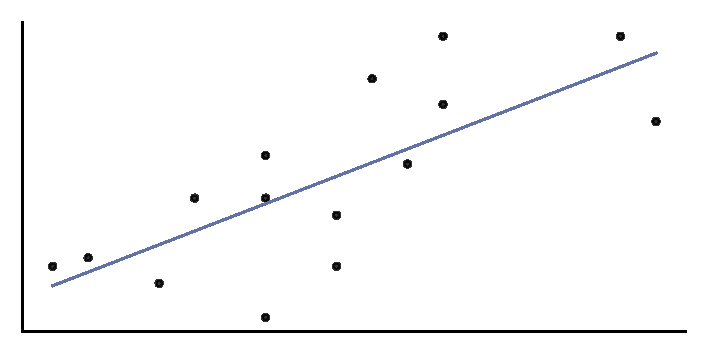
\includegraphics{figures/2review/nn/mae_chart.pdf}
    
    \fonte{prepared by the author.}
    \label{fig:mae_chart}
\end{figure}

\subsection{Optimizer}\label{sec:optimizer}

The optimizer is an algorithm that updates the model in response to the output of the loss function, that is, it aids to minimize the loss function. 
As the loss function minimizes, the model is getting closer to the target values and, hence, closer to the real pattern.

\subsubsection*{Gradient Descent} 

The \emph{gradient descent} is one of the main algorithm \cite{nesterov2004} that optimizes the model and many important ones are based on it, like the SGD. 
The goal is to get the minimum, as the error (loss) between the predicted and the target data is null. 
This would mean that the model fits to the pattern of the data.
%
\begin{figure}[!htb]
    \centering
    \caption[Gradient Descent Process]{Gradient Descent Process. Loss function can be represented in a two-axes plan. Depending on the data, it is not possible to represent graphically due to its multi dimension. Each point represents the learning step. When the gradient descent reaches the minimum of the loss function, it means that the model may be accurate. Note that the gradient descent can reach a local minimum of the function and not the global minimum necessarily. The \(y\)-axis represents the loss function and the \(x\)-axis represents the weight values. Red dot represents the minimum value of the loss function.}
    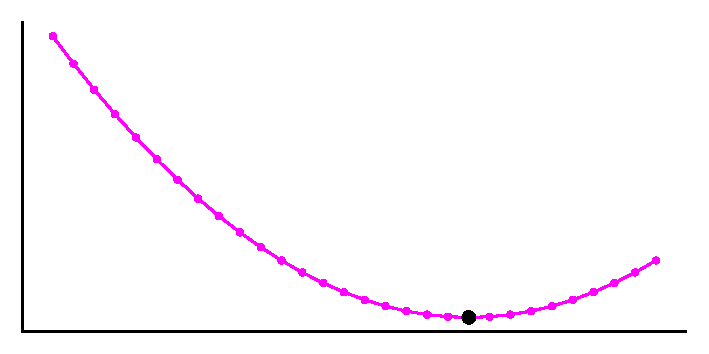
\includegraphics{figures/2review/nn/gradient_descent.pdf}
    
    \fonte{prepared by the author.}
    
\end{figure}

The gradient descent is a powerful algorithm that reduces the loss function, minimizing the error between the predicted value and the target value.

Since the gradient of a function gives the direction of the steepest ascent of a function and it is orthogonal to the surface at a determined point, it seems reasonable that moving in the perpendicular direction gives the maximum increase of the function \cite{stewart2016}.
On the other hand, the negative of the gradient may be used to find the opposite, that is, the steepest descent of the function, or the minimum decrease.
If the steps given to the direction of the negative gradient of the function are small, there is a good chance to get minimum value of the function.
However, if the steps are too long, the chance to pass by the minimum value is high \cite{nielsen2015}.
These steps are called \emph{learning rate} and should be chosen wisely.

This way, let \(\mathbf{x}\) be the entry vector with the predicted data and \(L\) the loss function adopted for some deep learning model, and \(\epsilon\) the learning rate, the gradient descent is:
%
\begin{equation}
    \mathbf{x}_{t+1} = \mathbf{x}_t - \epsilon \nabla L(\mathbf{x}_t)
\end{equation}

In determined cases, it is possible to avoid running the iterative algorithm and just go directly to the critical point by solving \(\nabla L(\mathbf{x}_t) = 0\) for \(\mathbf{x}\).

\subsubsection*{Stochastic Gradient Descent}

As seen, gradient descent is a powerful tool to minimize the loss function, however, for large data, the cost of operation is very high and its use is not feasible. 
The main idea of SGD is that the gradient is an expectation.
Later, the data is divided in subsets, also called \emph{mini-batch} and then the gradient is performed over them.
The mini-batch size is chosen to be a relatively small numbers of examples.
The data inside each subset may be considered redundant, that is why it uses one single value of the subset to compute the gradient descent.
This way, the process is considerable better for computational resources.

The SGD can be written as:
%
\begin{equation}
    \mathbf{x}_{t+1} = \mathbf{x}_t - \frac{\epsilon}{m} \sum_{i=1}^m \nabla L(\mathbf{x}_t; p^{(i)},q^{(i)})
\end{equation}
%
where \(m\)  is the mini-batch size; and \(\nabla L(\mathbf{x}; p^{(i)}, q^{(i)})\) is the gradient of the loss function with respect to the parameter vector \(\mathbf{x}\) for the \(i^{\text{th}}\) example \((p^{(i)}, q^{(i)})\) in the mini-batch.

Yet, nowadays, with the amount of data, many techniques are still applied in SGD as creating an automatic adaptive learning rates which achieve the optimal rate of convergence \cite{darken1991} and the momentum technique to improve it \cite{sutskever2013}.

\subsubsection*{Adam}

\emph{Adam}, shown in~\cref{alg:adam}, is an algorithm developed by \textcite{kingma2017} for first-order gradient-based optimization of stochastic objective functions, like the loss function, as seen in the~\cref{sec:loss_function}.
It is based on adaptive estimates of low-order moments and computationally efficient, requiring little computational memory.
Adam is a strategical choice when using large data or parameters and with very noisy/sparse gradients \cite{kingma2017}. 

\begin{algorithm}[!htb]
\captionsetup{labelfont={sf,bf}, labelsep=endash, font={footnotesize}}
\caption[Adam Algorithm]{Adam Algorithm. Good default setting are \(\alpha = 0.001,\ \beta_1 = 0.9,\ \beta_2 = 0.999\ \text{and}\ \epsilon = 10^{-8}\). Operations on vectors are element-wise.}
\begin{algorithmic}\footnotesize
\Require \(\alpha\): stepsize
\Require \(\beta_1,\ \beta_2\ \in [0,1)\): exponential decay rates for the moment estimates
\Require \(f(\theta)\): loss function
\Require \(\theta_0\): initial parameter

\State \(m_0 \gets 0\)
\State \(v_0 \gets 0\)
\State \(t \gets 0\)
\While{\(\theta_t\) not converged}
    \State{\(t \gets t + 1\)}
    \State{\(g_t \gets \nabla_{\theta}f_t(\theta_{t-1})\)}
    \State{\(m_t \gets b_1 \cdot m_{t-1} + (1-\beta_1) \cdot g_t\)}
    \State{\(v_t \gets \beta_2\cdot v_{t-1} + (1-\beta_2)\cdot g_t^2\)}
    \State{\(\widehat{m}_t \gets m_t/(1-\beta_1^t)\)}
    \State{\(\widehat{v}_t \gets v_t/(1-\beta_2^t)\)}
    \State{\(\theta_t \gets \theta_{t-1} - \alpha\cdot\widehat{m}_t/(\sqrt{\widehat{v}_t + \epsilon})\)}
\EndWhile

\Return \(\theta_t\)
\end{algorithmic}
\label{alg:adam}
\end{algorithm}